\documentclass[12pt,a4paper]{article}
\usepackage[utf8]{inputenc}
\usepackage{amsmath}
\usepackage{amsfonts}
\usepackage{amssymb}
\usepackage[margin = 1in, bottom=1in, top=1in]{geometry}
\usepackage{fancyhdr}
\usepackage{graphicx}
\usepackage{titlesec}
\usepackage{float}
\usepackage{amsmath}
\usepackage[utf8]{inputenc}
\usepackage[english]{babel}
\usepackage{siunitx}
\usepackage{hyperref}
\usepackage[all]{hypcap}
\usepackage[export]{adjustbox}
\usepackage{textcomp}
\usepackage{gensymb}
\usepackage{physics}
\usepackage[nottoc,notlot,notlof]{tocbibind}
\newcommand\tab[1][1cm]{\hspace*{#1}}
\parindent 0ex
\titleformat{\subparagraph}
    {\normalfont\normalsize\bfseries}{\thesubparagraph}{1em}{}
\titlespacing*{\subparagraph}{\parindent}{3.25ex plus 1ex minus .2ex}{.75ex plus .1ex}
\usepackage[acronym,nomain]{glossaries}
\usepackage{slashbox}
\usepackage[acronym]{glossaries}




\titleformat{\paragraph}
{\normalfont\normalsize\bfseries}{\theparagraph}{1em}{}
\titlespacing*{\paragraph}
{0pt}{3.25ex plus 1ex minus .2ex}{1.5ex plus .2ex}
\setcounter{secnumdepth}{4}
\setcounter{tocdepth}{4}

\renewcommand{\headrulewidth}{0pt}


\fancypagestyle{a}{\fancyhf[L]{
\includegraphics[scale=0.25]{1.png}}\fancyfoot[]}

\begin{document}

\begin{titlepage}
\begin{center}
\setcounter{page}{1}

\thispagestyle{a}
\vspace*{2cm}
\huge{\textbf{CIRCUIT DESIGN LAB WS 21/22}} \\[4mm]
\Large{\textbf{Ravensburg University of Applied Sciences}}\\ [1.5cm]

\line(1,0){450}\\
The Tea-Brewing-Controller \\
\line(1,0){450}\\ [0.75cm]




\begin{tabbing}
\hspace{6cm}\=\hspace{4.5cm}\=\kill
 Project By: \> Adil Azeez (34679)   \>  \\
  \> Gautam Sajeen (34636) \>   \\ \\
 Guided By: \>Dr.-Ing., Professor Walter Ludescher  \>    \\ 
   \\
 
   Submitted on:   \> 30.01.2022 \> 
\end{tabbing} 


\end{center}
\end{titlepage}

\newpage
\pagestyle{fancy}
\fancyfoot{}
\fancyhead{}

\setlength{\footskip=0pt}
\setlength{\headheight=35pt}

\newpage


\section*{Acknowledgement}

We are glad to express our indebtedness to our guide Prof. Dr. Walter Ludescher, Department of Electrical Engineering and Information Technology, Hochschule Ravensburg - Weingarten, for his constant guidance and help at all the stages of this project.\\

The objective of this project is to understand how a Circuit has to been designed using VHDL programming and implement it in the real world. The ultimate target is detect which mode has been selected and defining the timer range accordingly. Also the proper functionality of the Acoustic alarm has to be assured after the brewing process.\\





\newpage
\section*{Abstract}
In this Project, we have designed a circuit using VHDL (Very high-speed integrated circuit hardware description language) and FPGA (Field programmable gate array). A Tea Brewing Controller has been made with a variety of logical components efficiently connected to each other for a proper functionality. Basically, a Teabag has to be submerged in boiling water for some defined time ranging from two to five minutes. The system consists of a sensor which detected the teabag being dumped. It also monitors the time range and subsequently activates a buzzer. \\

Our project consists or two main components namely "Teabag-Sensor-Controller" and "Acoustic-Tea-Alarm". The TSC manages the sensor and detectes the time of arrival of the teabag. It also propagates this information to the ATA. The ATA reads the TOA data passes them to the transmitting part of the serial interface, using the ASCII code. It keeps track of the brewing process and activates the acoustic alarm signal when brewing has ended. \\

The circuit has been designed using VHDL. A block diagram of the Top Level Architecture and the Sound Component has been made to explain the entire functionality of the system. \\





\newpage
\pagestyle{fancy}
\fancyfoot{}
\fancyhead{}
\setlength{\footskip=25pt}
\setlength{\headheight=0pt}
%\renewcommand{\footrulewidth}{0.4pt}

\fancyfoot{}
\newpage

\rfoot{Page $\vert$ \thepage}
\pagenumbering{roman}
\setcounter{page}{5}
\tableofcontents
\clearpage

\section*{Section with acronyms}



\newacronym{gcd}{GCD}{Greatest Common Divisor}
\newacronym{lcm}{LCM}{Least Common Multiple}
\printglossary[type=\acronymtype]


\addcontentsline{toc}{section}{\listfigurename}
\listoffigures
\clearpage


\fancyfoot{}
\rfoot{\thepage}
\pagenumbering{arabic}
\setcounter{page}{1}
\renewcommand{\baselinestretch}{1.5} % line space
\section{Introduction}
In prder to design this circuitry, a few specific setups are necessary such as the Software setup for Simulation and Synthesis, Hardware Setup and uploading the code to the FPGA Board. This chapter contains the aforementioned details.  \

%\thispagestyle{c}
\subsection{Introduction to FPGA }
A Field Programmable Gate Array (FPGA) is a semiconductor device with programmable logic and interconnects. The programmable logic components can be used to replicate the functionality of fundamental logic gates like AND, OR, NOT, and XOR, as well as more advanced combinational operations like decoders and arithmetic functions. A hardware description language is used to specify the FPGA configuration (HDL). The most typical FPGA architecture comprises of a Configurable Logic Block (CLB) or Logic Array Block (LAB) array of logic blocks, I/O pads for off-chip connections, and programmable routing channels for logical function implementation. In addition to digital functions, FPGAs contain analogue features. Differential comparators on input pins designed to be coupled to differential signaling channels is a frequent analogue feature.\\

\begin{figure}[H]
\centering
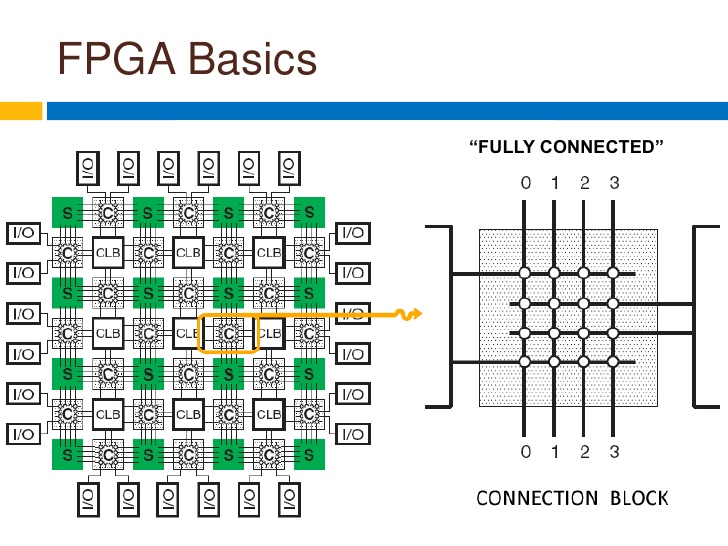
\includegraphics[height=10cm,width=11.5cm]{FPGA.jpg}
\caption{General Architecture of FPGA}
\label{General Architecture of FPGA}
\end{figure}
\newpage
\subsection{Introduction to the hardware used for the Project}
The following components are required to implement this project in reality:

\begin{figure}[H]
\centering
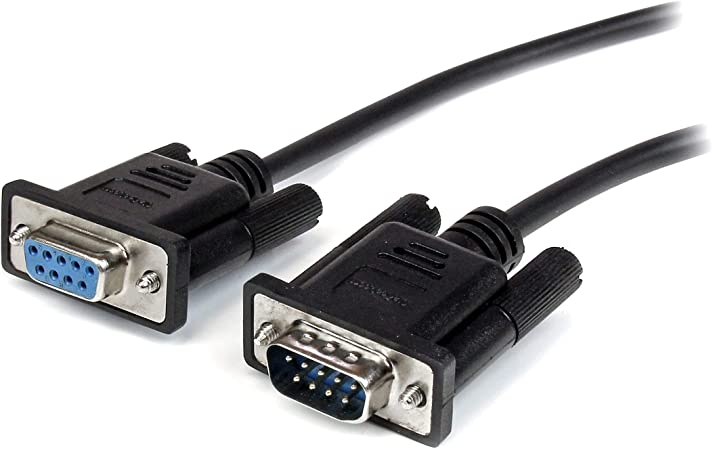
\includegraphics[width=6cm,height=5cm]{3wire.jpg}
\caption{Three wire Interface}
\label{Three wire Interface.jpg}
\end{figure}

\begin{figure}[H]
\centering
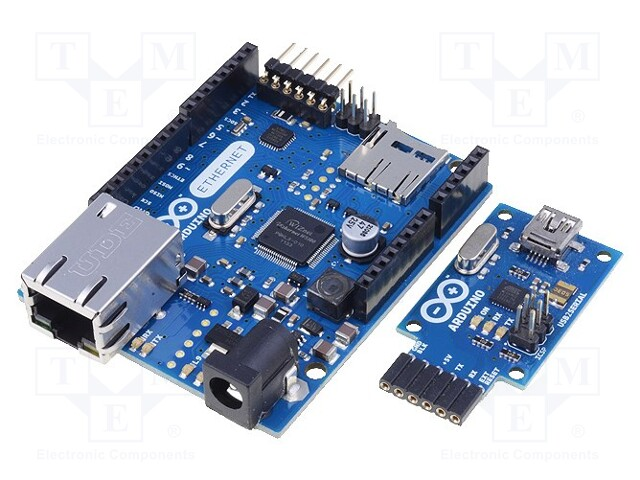
\includegraphics[width=6cm,height=5cm]{arduino.jpg}
\caption{Arduino Microcontroller}
\label{Arduino Microcontroller.jpg}
\end{figure}

\begin{figure}[H]
\centering
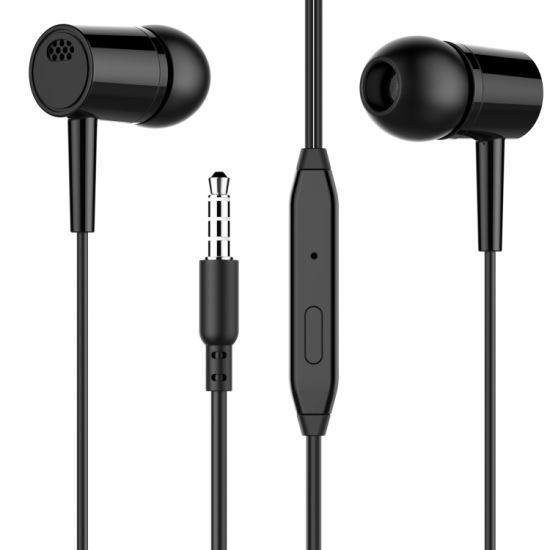
\includegraphics[width=6cm,height=5cm]{earphone.jpg}
\caption{Earphone}
\label{Earphone.jpg}
\end{figure}



\subsection{Information about VHDL}
VHDL stands for Very High-Speed Integration Circuit HDL (Hardware Description Language). It is an IEEE (Institute of Electrical and Electronics Engineers) standard hardware description language that is used to describe and simulate the behavior of complex digital circuits.\\
VHDL supports the following features:\
\begin{itemize}
\item Design methodologies and their features\
\item Sequential and concurrent activities \
\item Design exchange\
\item Standardization\
\item Documentation\
\item Readability\
\item Large Scale Design\
\item A wide range of descriptive capability\

\end{itemize} 

Why did we choose VHDL ? \
\begin{itemize}
\item It supports various design methodologies like Top-down approach and Bottom-up approach\
\item It provides a flexible design language\
\item It allows better design management\
\item It allows detailed implementations\
\item It supports a multi-level abstraction\
\item It provides tight coupling to lower levels of design\
\item It supports all CAD tools\
\item It strongly supports code re usability and code sharing\
\end{itemize} 

VHDL has constructs to handle the parallelism inherent in hardware designs, but these constructs (processes) differ in syntax from the parallel constructs in Ada (tasks). It is relatively easy for an inexperienced developer to produce code that simulates successfully but that cannot be synthesized into a real device, or is too large to be practical. One particular pitfall is the accidental production of transparent latches rather than D-type flip-flops as storage elements.\\

One can design hardware in a VHDL IDE (for FPGA implementation such as Xilinx ISE, Altera Quartus, Synopsys Synplify or Mentor Graphics HDL Designer) to produce the RTL schematic of the desired circuit. After that, the generated schematic can be verified using simulation software which shows the waveforms of inputs and outputs of the circuit after generating the appropriate testbench. To generate an appropriate testbench for a particular circuit or VHDL code, the inputs have to be defined correctly. For example, for clock input, a loop process or an iterative statement is required.\\

A final point is that when a VHDL model is translated into the "gates and wires" that are mapped onto a programmable logic device such as a CPLD or FPGA, and then it is the actual hardware being configured, rather than the VHDL code being "executed" as if on some form of a processor chip.\\





\newpage

\renewcommand{\baselinestretch}{1.5} % line space
\section{CIRCUIT DESIGNING WITH VHDL}
A brief overview of the top level of the Circuit blocks will be described in this chapter. Moreover, the top level consists of some small blocks such as counters, multiplexers,etc is going to described in this chapter.\\


\subsection{Top Level Block Diagram Entity}

\begin{figure}[H]
\centering
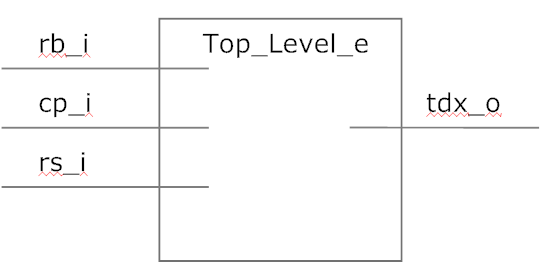
\includegraphics{TopLevelE.JPG}
\caption{Top Level Entity}
\label{Top Level Entity}
\end{figure}


\begin{enumerate}
\item \textbf{cp\_i:} cp\_i denotes the system clock. It is a continuous sequence of low and High on the line providing to it. The system clock is needed to synchronize all the components that is running on the FPGA board. That means, they all do their work only if the clock is high;never when it’s low. And because of the clock speed is set above the longest time any signal needs to propagate through any circuit on the board,this signals is preventing signals from arriving before other signals and thus makes everything safe and synchronized.

\item \textbf{rb\_i:} rb\_i denotes the reset button signal. It is an active low signal. It is a signal that initialize the complete system. Reset can be switch button or a push button and is generally used by the user. It restart all the interfaces and all the State Machines which are working inside the FPGA chip, are forced to go to its initial state. 

\item \textbf{st\_i:} st\_i is the signal that is coming from the sensor, that is activated when the Teabag is dipped in the boiling water. As soon as the teabag is dipped, the sensor is set to active high untill the Teabag stays in the water and the Alarm starts ringing. Therefore this signal is collected by the TSC and propagated towards the ATA.

\item \textbf{txd\_o:} txd\_o is the signal that send a serial line of data that is processed inside the system. That means, the data that comes are the bits that are sent in UART sequence corresponding to the RS-232 Protocol.

\end{enumerate}

Here, the signals from the top\_level entity have been discussed. The Architecture is declared and explained in the next Section.\

\begin{figure}[H]
\centering
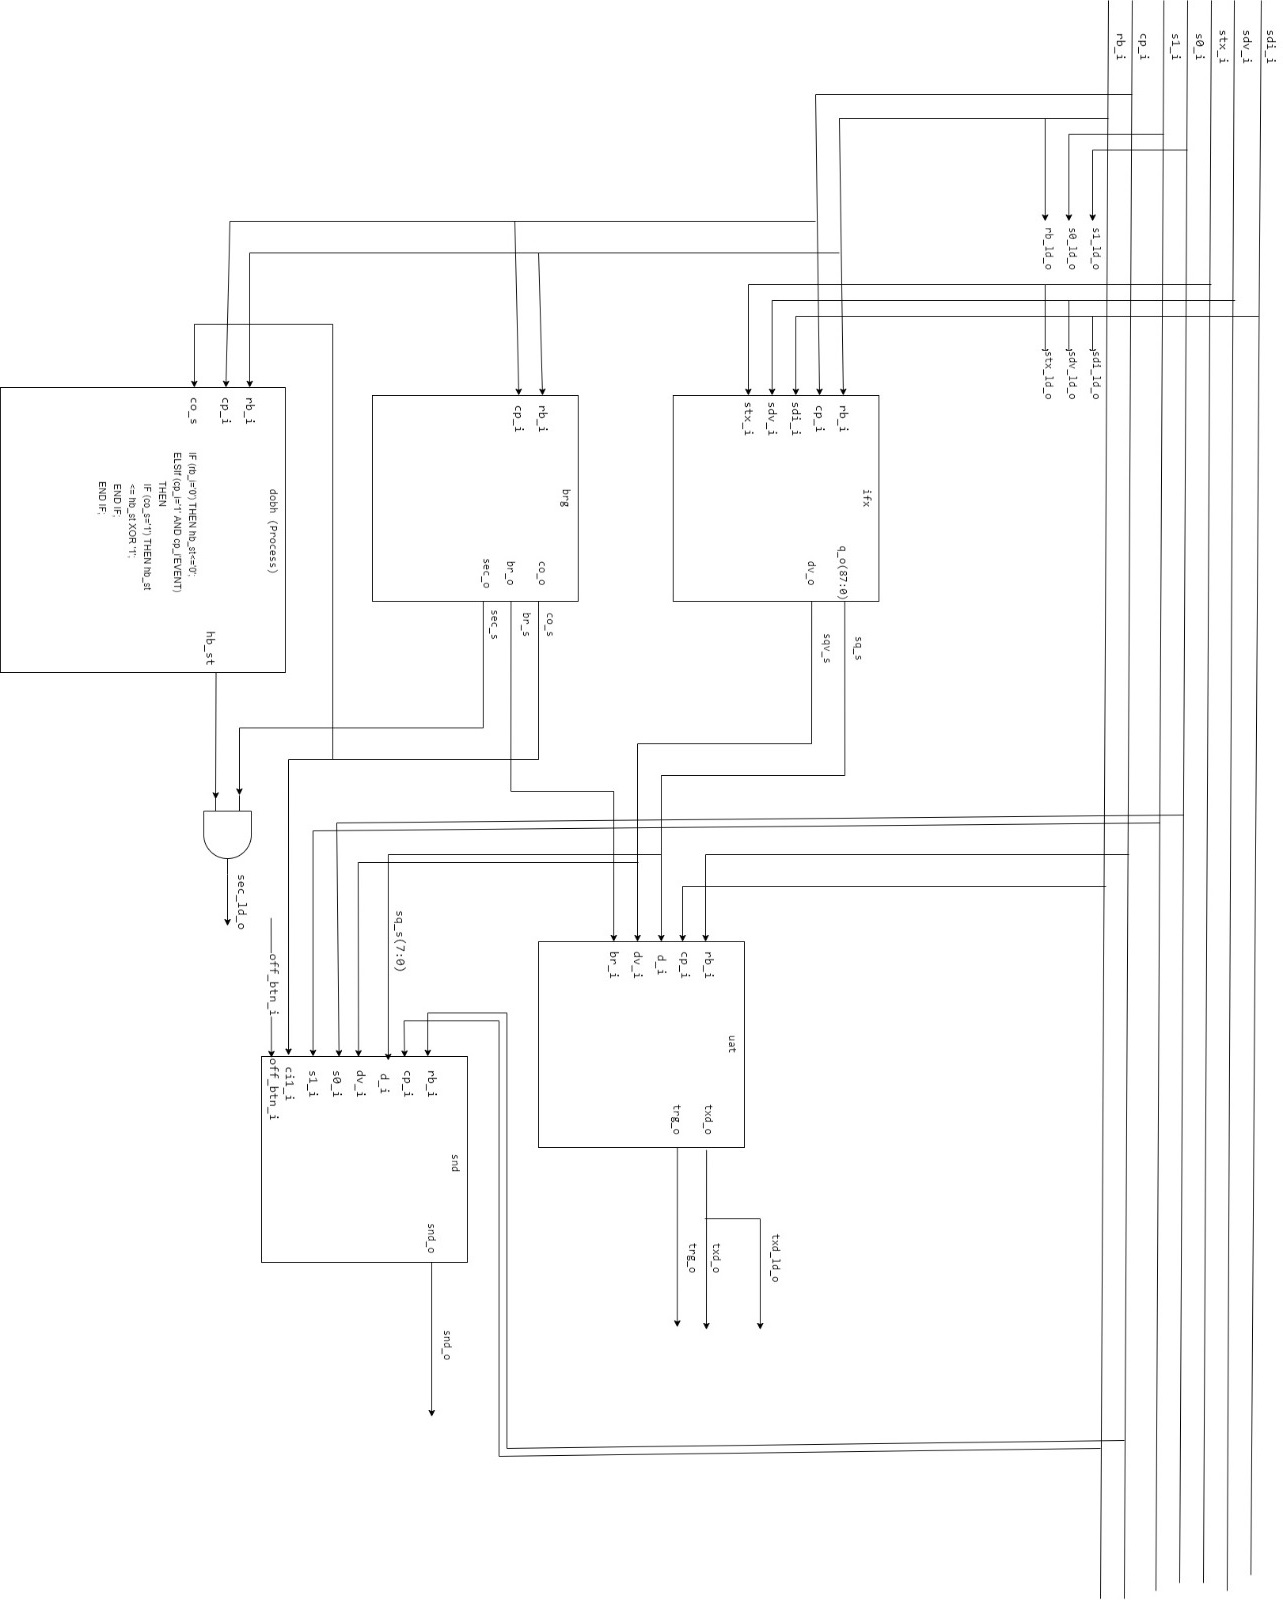
\includegraphics [width=16cm,height=23cm]{Top.jpg}
\caption{Top Level Architecture}
\label{Top Level Architecture}
\end{figure}
\newpage




\subsection{ifx}
The entity of the ifx looks like :\\

\begin{figure}[H]
\centering
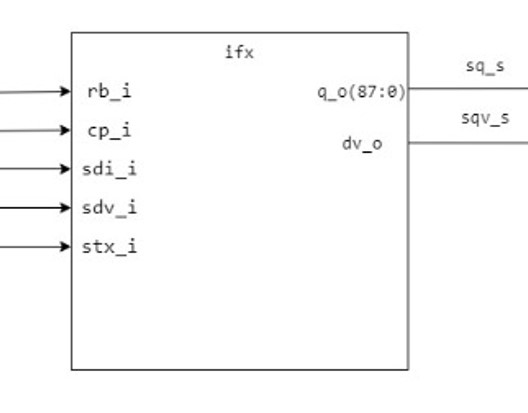
\includegraphics[width=8cm,height=6cm]{ifx_ss.jpg}
\caption{ifx Entity}
\label{ifx Entity}
\end{figure}

This block is responsible for handling the serial input. It accepts the data serially from the outside world. rb\_i is the reset bit. cp\_i is the clock pulse. sd\_i is serial data, sdv\_i is serial data valid , stx\_i basically starts the transmission. The output q\_0 transmits the data as a standard logic vector of 87 down to 0. dv\_o is associated with validity of the data. 

\subsection{brg}
The entity of the Baudrate Generator looks like :\\

\begin{figure}[H]
\centering
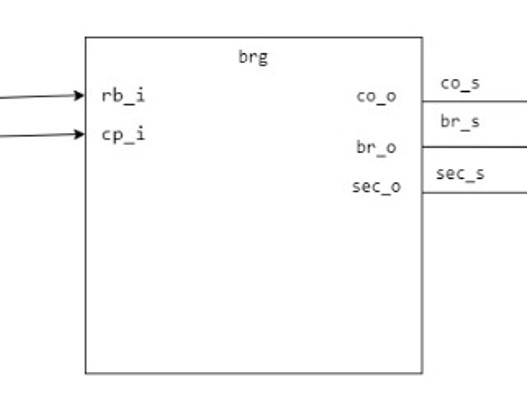
\includegraphics[width=8cm,height=6cm]{brg_ss.jpg}
\caption{Baudrate Generator Entity}
\label{Baudrate Generator Entity}
\end{figure}

This block is responsible for generating the Baudrate. rb\_i is the reset bit. cp\_i is the clock pulse. It outputs the baudrate, the one second signal and the one second carry out. 


\subsection{uat}
The entity of the Transmission looks like :\\

\begin{figure}[H]
\centering
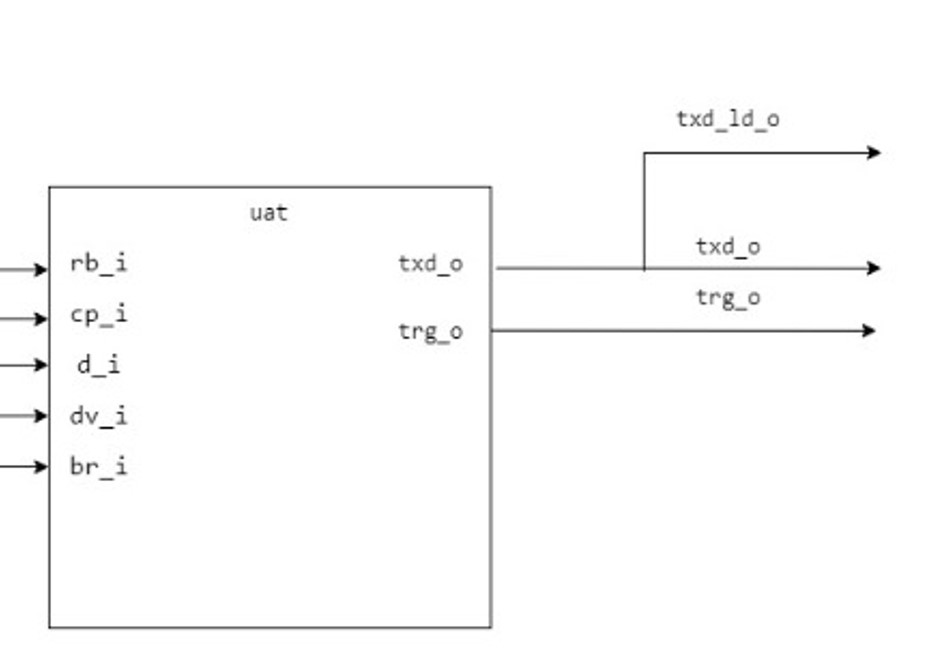
\includegraphics[width=8cm,height=6cm]{uat_ss.jpg}
\caption{uat Entity}
\label{uat Entity}
\end{figure}

This block is responsible for transmitting the data to the outside world.  rb\_i is the reset bit. cp\_i is the clock pulse. d\_i is data which is needed to be transmitted. dv\_i is the validity of the data. txd\_o transmits the data serially. trg\_o represents the slope at the start bit. 

\subsection{snd}
The entity of the Sound Generator looks like :\\

\begin{figure}[H]
\centering
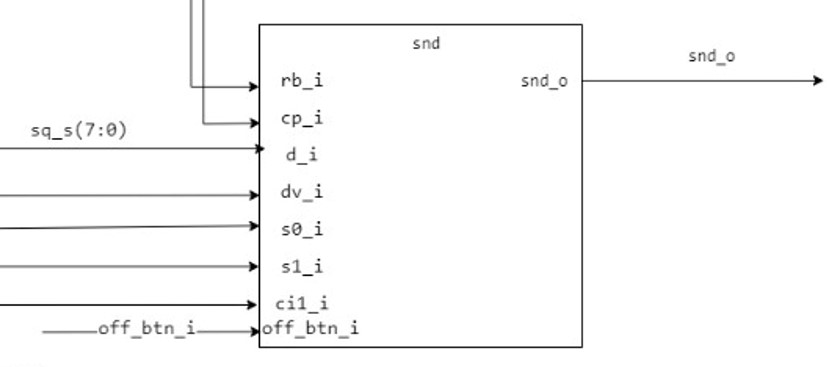
\includegraphics[width=12cm,height=6cm]{newsnd_ss.jpg}
\caption{snd Entity}
\label{snd Entity}
\end{figure}

This block is responsible for the sound generation.  rb\_i is the reset bit. cp\_i is the clock pulse. d\_i is data which is needed to be transmitted. dv\_i is the validity of the data. s0\_i and s1\_i are responsible for the mode selection. ci1\_i represents the one second pulse. snd\_o is the final sound output. 













\begin{figure}[H]
\centering
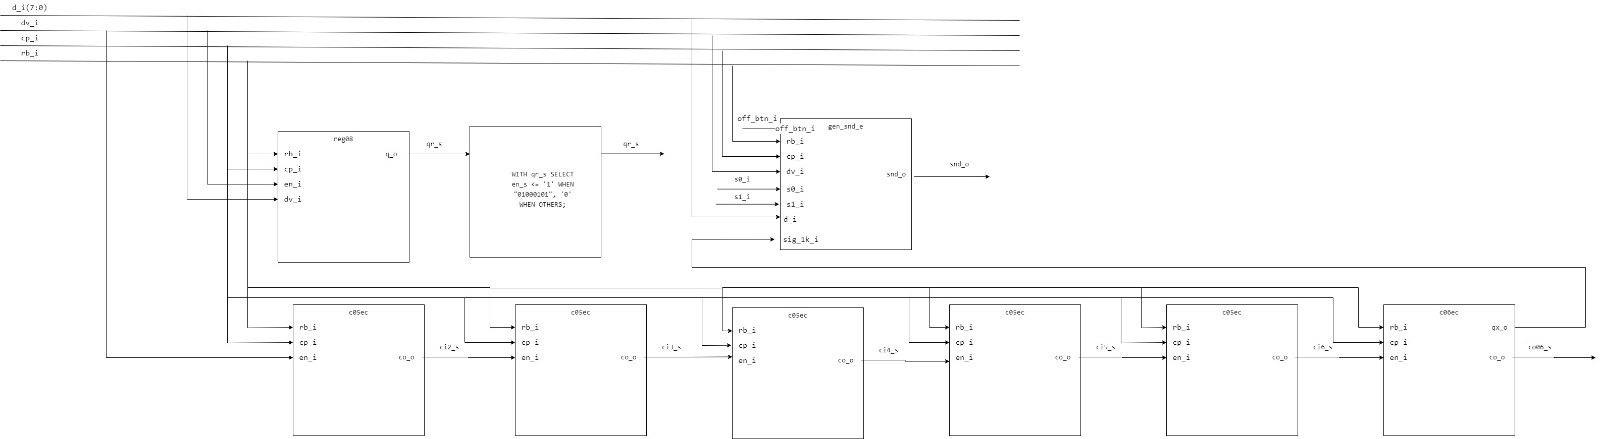
\includegraphics[width=18cm,height=6cm]{new.jpeg}
\caption{The architecture of the Sound Component}
\label{The architecture of the Sound Component}
\end{figure}


\textbf{Sound Component:} In this Block Diagram, c05ec and co6ec are used to generate the 1kHz signal. Thereafter, all the signals are driven to the gen\_snd\_e. This block consists of an FSM and generates the sound depending on the selected mode.
The FSM has been given below. 


\begin{figure}[H]
\centering
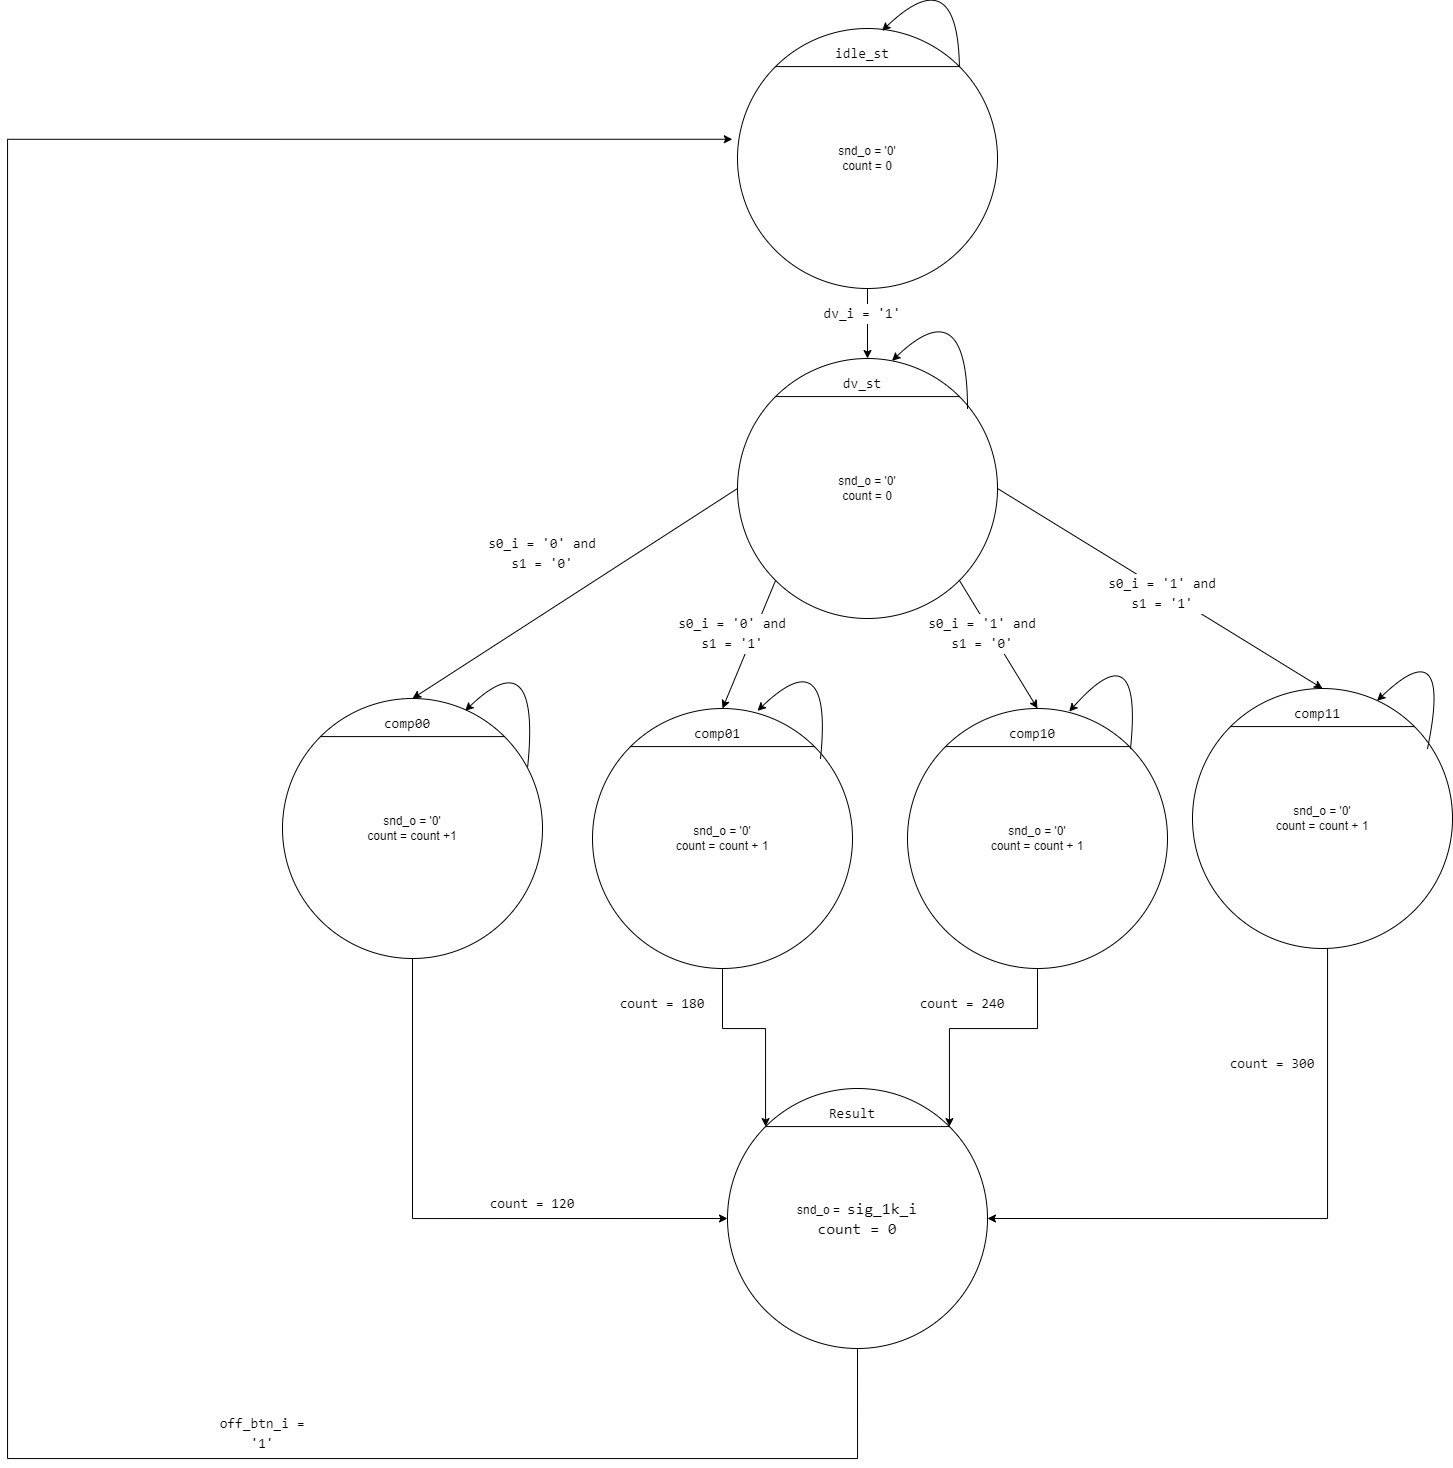
\includegraphics[scale=0.35]{FSM.jpeg}
\caption{The Finite State Machine of the Sound Component}
\label{The Finite State Machine of the Sound Component}
\end{figure}


 \textbf{Sound FSM:} When the FSM starts, it is in ideal state. When dv\_i signal is detected, the transition occurs to state dv\_st. Now depending on the mode selected, it correspondingly goes to comp00 or comp01 or comp10 or comp11. For example, the mode for 2 minutes is selected, then it is directed towards the comp00 state. It waits in that respective state until the count is equal to 120. Count is constantly getting incremented at every second pulse. So 120 second pulses mean 2 minutes. Thereafter, it is driven to the result state where the sound is generated. Once the OFF button is pressed, then only it goes to the ideal state, otherwise the sound is constantly generated. 



\newpage


\raggedright

\newpage                                                                                %biblography
%\section{Reference}
\begin{thebibliography}{}

\bibitem{Intro1}
\texttt{<https://en.wikipedia.org/wiki/Field-programmable\_gate\_array>}

\bibitem{Intro3}
\texttt{<https://en.wikipedia.org/wiki/VHDL>}



\end{thebibliography}



\clearpage

\end{document}
